% !TEX root = ../../prj4projektdokumentation.tex

\subsection{Analog til digital konvertering}

Måleenheden omsætter to analoge spændingssignaler til digitale værdier for strøm og spænding. Denne konvertering foretages af en Delta Sigma Analog to Digital Converter (ADC) i PSOCen (REFERENCE-adc datblad).  ADC er en komponent i PSOC, som med en read-funktion kan returnere en 16-bit værdi af det analoge signal op indgangen. 

På Figur \ref{fig:MEADC} ses blokkaldet i PSOC creator 4.0. Blokken er sat op med følgende parametre:

\begin{align}
Resolution = 16bit
\end{align}

\begin{align}
f_{sample} = 41666 Hz
\end{align}

\begin{figure}[htbp] % (alternativt [H])
	\centering
	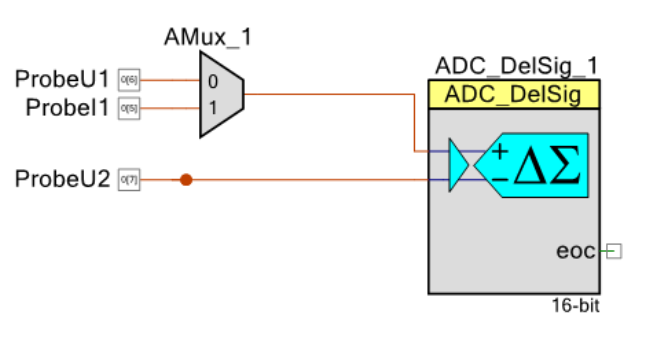
\includegraphics[width=0.6\textwidth]{Figure/MEADC}
	\caption{ADC blok fra PSOC creator 4.0}
	\label{fig:MEADC}
\end{figure}

Som det fremgår af Figur \ref{fig:MEADC} er der anvendt 2 multiplexere, til at skifte mellem hvilke signaler der skal samples. Dette skyldes at der kun er én ADC i PSOCen. Samplingen af signalet styres i C-koden, hvor der anvendes to af ADC-blokkens API funktioner. 
\\

\textbf{GetResult16() }starter en ADC konvertering, venter på at denne er færdig, stopper konverteringen og returnerer en 16bit signed int værdi af resultatet. 
\\

\textbf{CountsTo\_mVolt()} konverterer resultatet af GetResult16() til en værdi i millivolt. 
\\

Koden til sampling af signalerne er vist grafisk i et flowchart i Figur \ref{fig:MEsample}. Samplingen kører i en for-løkke, hvor der skiftevis tages et sample af spændingen og strømmen. Efter hver anden sample, indføres der et delay, således at sampletiden passer med én periode af det 50Hz sinussignal. Antallet af samples er 64 pr. signal, altså 128 i alt. De samplede værdier gemmes i to arrays, som bruges i de efterfølgende beregninger. 


\begin{figure}[htbp] % (alternativt [H])
	\centering
	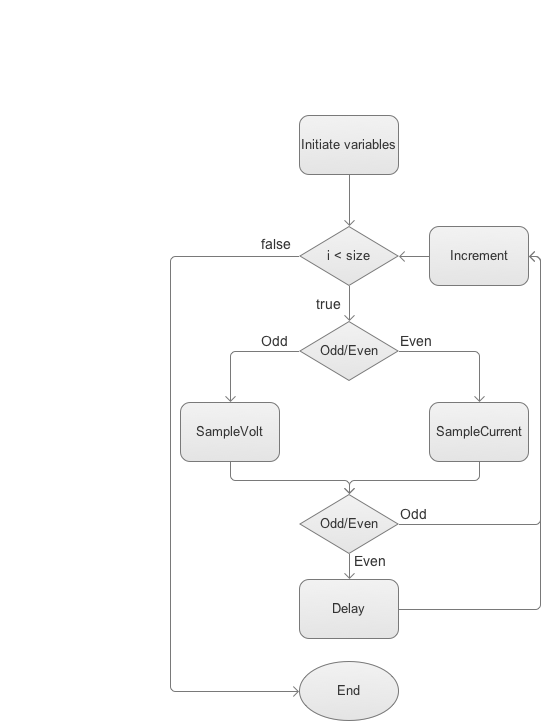
\includegraphics[width=0.6\textwidth]{Figure/MEsample}
	\caption{Flowchart for sample funktionen i PSOC}
	\label{fig:MEsample}
\end{figure}

\subsubsection{Realisering af samplefrekvens}

Det indførte delay i for-løkken skal sikre at sampletiden svarer præcist til én periode af det 50Hz sinussignal.
\begin{align}
T_{sample} = \frac{1}{50Hz} = \SI{20}{\milli\second}
\end{align}

Det betyder at tiden mellem hvert sample skal være
\begin{align}
t = \frac{T_{sample}}{128} = \SI{156,25} {\micro\second}
\end{align}

Ved at sætte et udgangsben på PSOC højt lige inden der tages et sample, og sætte det lavt igen lige inden næste sample, er tiden mellem samples, uden delay, aflæst til $t = \SI{131,81}{\milli\second}.$


